\documentclass[10pt]{beamer}

%-------------------------------------------------------
% Beamer Theme location override
%-------------------------------------------------------

\makeatletter
  \def\beamer@calltheme#1#2#3{%
    \def\beamer@themelist{#2}
    \@for\beamer@themename:=\beamer@themelist\do%
    {\usepackage[{#1}]{\beamer@themelocation/#3\beamer@themename}}}

  \def\usefolder#1{
    \def\beamer@themelocation{#1}
  }
  \def\beamer@themelocation{}

%-------------------------------------------------------
% INCLUDE PACKAGES
%-------------------------------------------------------

\usepackage{listings} % Code listing old style
% \usepackage{minted} % Code listing new style
% \usepackage{forest} % Tree graphs
\usepackage{fontspec} % UTf-8 input support
% \usepackage{multirow}
\usepackage{hyperref} % Style links
\usepackage{wasysym}
\usepackage[absolute,overlay]{textpos}
\usepackage{graphicx}
\usepackage{microtype} % nice text appearance
\usepackage{ragged2e}
\usepackage{pgfpages}
\usepackage[ngerman]{babel}
\usepackage{docmute} % Import other .tex files ignoring document
% \usepackage{multicol} % Automatically use multiple columns
\usepackage{fontawesome} % WebFonts including href icon

%-------------------------------------------------------
% Config Theme
%-------------------------------------------------------
\usefolder{../Templates/featherZR}
\usetheme[
    progressstyle=movingCircCnt   % fixedCircCnt, movingCircCnt (moving is deault)
  ]{Feather}

  \setsansfont{HelveticaNeue}
  \setmonofont{Source Code Pro for Powerline}[Scale = MatchLowercase]

%-------------------------------------------------------
% DEFFINING AND REDEFINING COMMANDS
%-------------------------------------------------------

\setbeameroption{show notes}
\setbeameroption{show notes on second screen=right}

%Set Path to images
\graphicspath{{Images/}}

% colored hyperlinks
\newcommand{\chref}[2]{%
\href{#1}{{\usebeamercolor[bg]{Feather}#2} {\footnotesize\faExternalLink}}%
}

%Justification
\addtobeamertemplate{theorem begin}{}{\justifying}
\addtobeamertemplate{block begin}{}{\justifying}
\addtobeamertemplate{itemize begin}{}{\justifying}
\addtobeamertemplate{item begin}{}{\justifying}
\addtobeamertemplate{frame begin}{}{\justifying}
\addtobeamertemplate{quote begin}{}{\justifying}
\addtobeamertemplate{structure begin}{}{\justifying}

%etoolbox für nested list covering
\setbeamercovered{transparent}

%description inde
\setbeamersize{description width=0.57cm}

\makeatletter
\newcommand*\fix@beamer@close{%
  \ifnum\beamer@trivlistdepth>0
  \beamer@closeitem%
  \fi
}
\newcommand*\fix@beamer@open{%
  \ifnum\beamer@trivlistdepth>0
  \gdef\beamer@closeitem{}%
  \fi
}
\newcommand<>{\highlighton}[1]{%
  \alt#2{\structure{#1}}{{#1}}
}


\BeforeBeginEnvironment{enumerate}{\fix@beamer@close}
\AfterEndEnvironment{enumerate}{\fix@beamer@open}
\BeforeBeginEnvironment{itemize}{\fix@beamer@close}
\AfterEndEnvironment{itemize}{\fix@beamer@open}
\BeforeBeginEnvironment{description}{\fix@beamer@close}
\AfterEndEnvironment{description}{\fix@beamer@open}
\makeatother

% Codelistings
\lstset{language=bash,
	basicstyle=\footnotesize\ttfamily,
	keywordstyle=\color{blue},
	stringstyle=\color{red},
	commentstyle=\color{gray},
	breaklines=true,
	tabsize=2
}

%-------------------------------------------------------
% INFORMATION IN THE TITLE PAGE
%-------------------------------------------------------

\title[Git ] % [] is optional - is placed on the bottom of the sidebar on every slide
{ % is placed on the title page
      \textbf{Git}
}

\subtitle[ -- Funktionsweise von Git]
{
%      \textbf{v. 1.0.0}
}

\author[Sebastian Knott]{Sebastian Knott}

\institute[]
{
      ZooRoyal IT\\

  %there must be an empty line above this line - otherwise some unwanted space is added between the university and the country (I do not know why;( )
}

\date{\today}

%-------------------------------------------------------
% THE TITLE OF THE PRESENTATION
%-------------------------------------------------------

\begin{document}

{\1
\begin{frame}[plain,noframenumbering] % the plain option removes the header from the title page, noframenumbering removes the numbering of this frame only
  \titlepage% call the title page information from above
\end{frame}}

% \AtBeginSection[]
% {
%   \frame<handout:0>
%   {
%     \frametitle{Überblick}
%     \tableofcontents[currentsection,hideothersubsections,sectionstyle=show/shaded,subsectionstyle=show/shaded]
%   }
% }

\AtBeginSubsection[]
{
  \frame<handout:0>
  {
    \frametitle{Überblick}
    \begin{columns}
      \begin{column}{0.5\textwidth}
        \begin{figure}
          \begin{center}
            
\includegraphics[width=\textwidth]{git_logo}
          \end{center}
        \end{figure}
      \end{column}
      \begin{column}{0.5\textwidth}
        \tableofcontents[currentsection,hideothersubsections,sectionstyle=show/shaded,subsectionstyle=show/shaded]
      \end{column}
    \end{columns}
  }
}

\AtBeginSubsubsection[]
{
  \frame<handout:0>
  {
    \frametitle{Überblick}
    \begin{columns}
      \begin{column}{0.5\textwidth}
        \begin{figure}
          \begin{center}
            
\includegraphics[width=\textwidth]{git_logo}
          \end{center}
        \end{figure}
      \end{column}
      \begin{column}{0.5\textwidth}
        \tableofcontents[currentsection,hideothersubsections,sectionstyle=show/shaded,subsectionstyle=show/shaded,subsubsectionstyle=show/shaded]
      \end{column}
    \end{columns}
  }
}

%-------------------------------------------------------
% THE BODY OF THE PRESENTATION
%-------------------------------------------------------

\begin{frame}
  \frametitle{Überblick}
  \begin{columns}
    \begin{column}{0.5\textwidth}
      \begin{figure}
        \begin{center}
          
\includegraphics[width=\textwidth]{git_logo}
        \end{center}
      \end{figure}
    \end{column}
    \begin{column}{0.5\textwidth}
      \tableofcontents[currentsection,sectionstyle=show,subsectionstyle=show,subsubsectionstyle=hide]
    \end{column}
  \end{columns}
\end{frame}


\section{Git unter der Haube}
\subsection{Datenhaltung in Git}


\begin{frame}[<+->]
  \frametitle{Datenhaltung in Git}
  \framesubtitle{Versionen und Dateien}

  \begin{figure}
        \begin{center}
          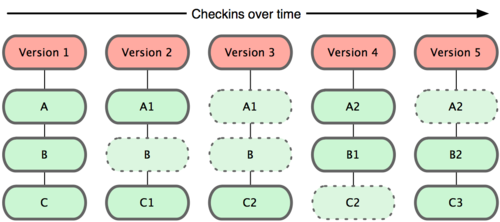
\includegraphics[width=\textwidth]{git_file_store_strategy}
        \end{center}
  \end{figure}
  \begin{itemize}
    \item Git speichert in jedem Commit die Dateien als ganzes
      \note[item]{Entspricht cp -r quelle ziel}
    \item Unveränderte Dateien werden allerdings nur referenziert
  \end{itemize}
\end{frame}


\begin{frame}<handout:0>[label=fragen]
  \frametitle{Fragen}
  \framesubtitle{Fragen?}
  \begin{figure}
    \begin{center}
      
\includegraphics[height=4cm]{fragen}
    \end{center}
  \end{figure}
\end{frame}


\begin{frame}
  \frametitle{Datenhaltung in Git}
  \framesubtitle{Git Objekte}

  \begin{columns}[onlytextwidth]
  	\begin{column}{0.5\textwidth}
      \begin{block}<+->{}
        Git kennt vier Typen von Objekten
        \begin{description}[commit]
          \item[blobs] Dateien
          \item[trees] Verzeichnisse
          \item[commit] Momentaufnahmen des Workspace
          \item[tags] signierte Namen von commits
        \end{description}
      \end{block}
      \begin{block}<+->{}
          Alle Objekte werden mit einem SHA-1 Hash ihres Inhalts identifiziert
      \end{block}

    \end{column}
    \begin{column}{0.5\textwidth}
      \begin{figure}
        \begin{center}
          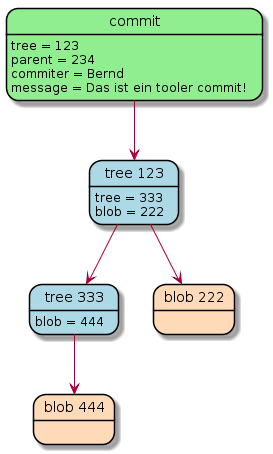
\includegraphics[height=6cm]{commit}
        \end{center}
      \end{figure}
    \end{column}
  \end{columns}

\end{frame}


\againframe<handout:0>{fragen}

\note{Aufgabe: Verzeichnisbaum anzeichnen und neuen Git Commit mit Verzeichnissen und Datien konstruieren lassen.}


\subsection{History}


\begin{frame}[<+->]
  \frametitle{History}
  \framesubtitle{Verkettung von commits}

  \begin{figure}
        \begin{center}
          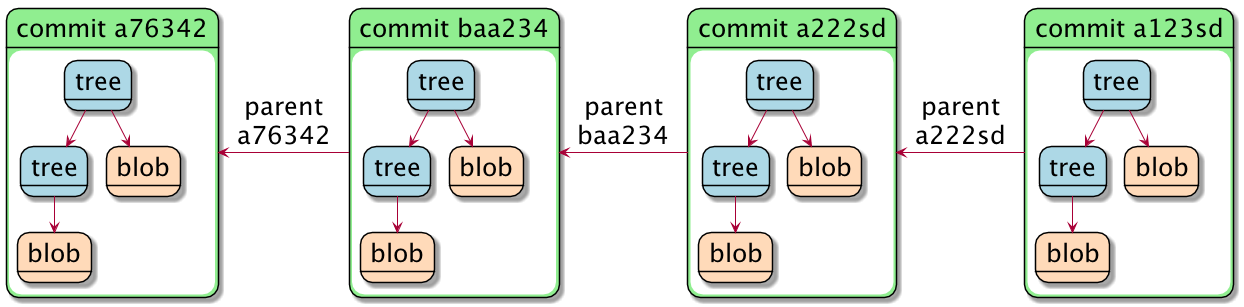
\includegraphics[width=\textwidth]{history}
        \end{center}
  \end{figure}
  \begin{itemize}
    \item Alle Dateien, Ordner, Commits werden in Git-Objekten verwaltet
    \item Die Git-Objekte bilden eine Baumstruktur
  \end{itemize}
  \note[item]{Aufgabe: Commit anzeichnen. Eine Datei verändert. Neuen Commit anzeichnen lassen.}
\end{frame}


\againframe<handout:0>{fragen}


\subsection{Branch}


\begin{frame}
  \frametitle{Branches}
  \framesubtitle{Organisation von Commits}

  \begin{columns}[onlytextwidth]
    \begin{column}{0.5\textwidth}
      \begin{itemize}
        \item Branches sind Pointer auf commits
        \item Verschiedene Commit-ishs für gleichen Commit \\
              \lstinline|git checkout 78aca6| \\
              \lstinline|git checkout master| \\
              \vspace{0.5em}
              (\alert{Vorsicht}! Detached Head!)
      \end{itemize}

    \end{column}
    \begin{column}{0.5\textwidth}
      \begin{figure}
        \begin{center}
          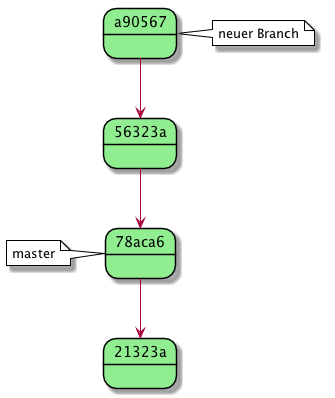
\includegraphics[height=6cm]{branch1}
        \end{center}
      \end{figure}
    \end{column}
  \end{columns}
\end{frame}


\begin{frame}
  \frametitle{Branches}
  \framesubtitle{Organisation von Commits}

  \begin{columns}[onlytextwidth]
    \begin{column}{0.5\textwidth}
      Neue commits in einem Branch verschieben den Pointer
    \end{column}
    \begin{column}{0.5\textwidth}
      \begin{figure}
        \begin{center}
          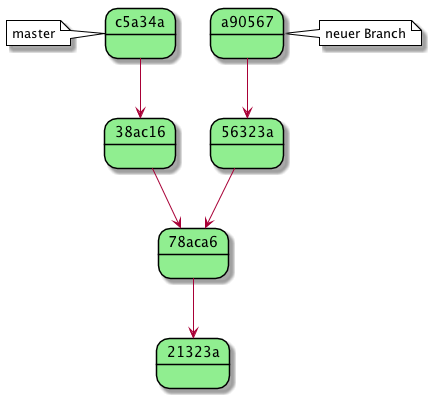
\includegraphics[width=\textwidth]{branch2}
        \end{center}
      \end{figure}
    \end{column}
  \end{columns}
\end{frame}

\note[itemize]{
  \item Aufgabe1: Git Commit anzeichnen. Weitere Branches erzeugen lassen. Weitere Commits erzeugen lassen. Einen Branch resetten.
  \item Hashes verändern sich nicht!
}


\againframe<handout:0>{fragen}


\subsection{Merge}


\begin{frame}
  \frametitle{Merge}
  \framesubtitle{Zusammenführen von zwei Branches}

  \begin{columns}[onlytextwidth]
    \begin{column}{0.5\textwidth}
      \begin{itemize}
        \item<+-> Neuer Branch $\rightarrow$ master
        \item<+-> Quellbranch bleibt bestehen
        \item<+-> Pointer im Quellbranch wird nicht bewegt
        \item<+-> Neuer commit (\lstinline|cda323|) hat zwei Parents
          \note[item]{Mit HEAD~1 wird uneindeutig. HEAD\^{}1 gibt Parent an}
        \item<+-> \lstinline|git branch -d neuer Branch| entfernt nur den Pointer, nicht die commits
      \end{itemize}
    \end{column}
    \begin{column}{0.5\textwidth}
      \begin{figure}
        \begin{center}
          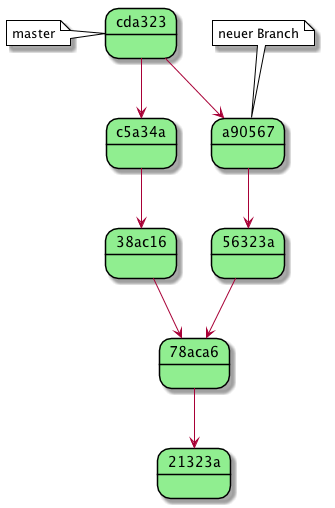
\includegraphics[height=6cm]{merge}
        \end{center}
      \end{figure}
    \end{column}
  \end{columns}
\end{frame}


\begin{frame}
  \frametitle{Merge}
  \framesubtitle{Mergen mit Fast Forward}

  \begin{columns}[onlytextwidth]
    \begin{column}{0.3\textwidth}
      \begin{figure}
        Vorher
        \begin{center}
          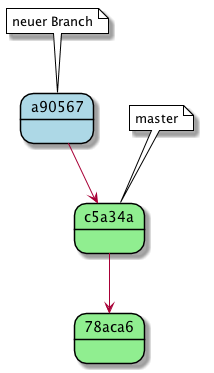
\includegraphics[width=\textwidth]{merge_pre_fast_forward}
        \end{center}
      \end{figure}
    \end{column}
    \begin{column}{0.3\textwidth}
      \begin{center}
      Entspricht Rebase + Reset master
      \vspace{1em}
      \begin{itemize}
        \item Pointer wird weiter geschoben
        \item Nur ein Parent
        \item Lineare History
        \item Git Default
      \end{itemize}
      \end{center}
    \end{column}
    \begin{column}{0.3\textwidth}
      \begin{figure}
        Nachher
        \begin{center}
          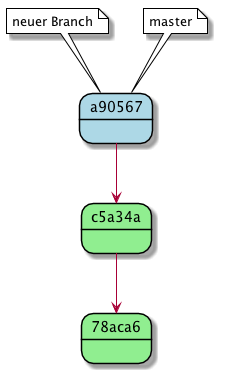
\includegraphics[width=\textwidth]{merge_post_fast_forward}
        \end{center}
      \end{figure}
    \end{column}
  \end{columns}
\end{frame}


\againframe<handout:0>{fragen}


\subsection{Rebase}


\begin{frame}
  \frametitle{Rebase}
  \framesubtitle{Was passiert bei einem Rebase}

  \begin{columns}[onlytextwidth]
    \begin{column}{0.3\textwidth}
      \begin{figure}
        Vorher
        \begin{center}
          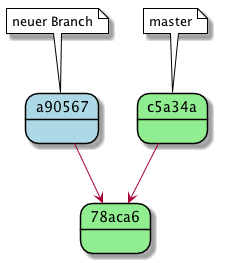
\includegraphics[width=\textwidth]{rebase_pre}
        \end{center}
      \end{figure}
    \end{column}
    \begin{column}{0.3\textwidth}
      \begin{center}
      \begin{itemize}
        \item Commit wird kopiert und Parent gesetzt
        \item master Pointer wird \alert{nicht} verschoben
        \item Lineare History
      \end{itemize}
      \end{center}
    \end{column}
    \begin{column}{0.3\textwidth}
      \begin{figure}
        Nachher
        \begin{center}
          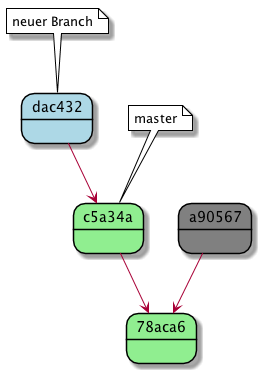
\includegraphics[width=\textwidth]{rebase_post}
        \end{center}
      \end{figure}
    \end{column}
  \end{columns}
\end{frame}


\begin{frame}[<+->]
  \frametitle{Rebase}
  \framesubtitle{Interaktive Rebases}
  Rebase gibt einem weitere Möglichkeiten Commits umzuorganisieren.
  \begin{description}[Squash, Fixup]
    \item[Drop] Einzelne Commits entfernen
    \item[Squash, Fixup] Commits zusammenführen
    \item[Reword] Einzelne Commit Messages ändern
    \item[Edit] Einzelne Commits amenden
  \end{description}
  Operationen können beliebig kombiniert werden
\end{frame}


\begin{frame}
  \frametitle{Rebase}
  \framesubtitle{Mächtiges Rebase}
  \begin{columns}[onlytextwidth]
  \begin{column}{0.5\textwidth}
  \begin{figure}
    \begin{center}
      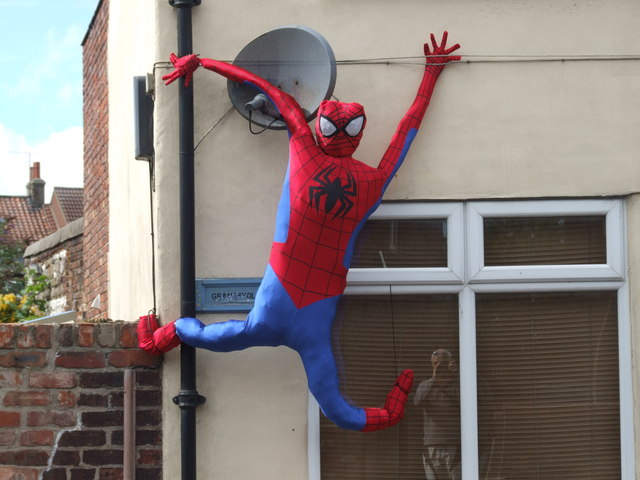
\includegraphics[width=\textwidth]{spiderman}
    \end{center}
    Mit großer Macht kommt große Verwirrung
  \end{figure}
  \end{column}
  \begin{column}{0.5\textwidth}
    \begin{itemize}
      \item Vorsicht vor Branches, auf denen andere Entwickler Arbeiten
      \item Überkomplexe Branches machen Rebases extrem schwer
      \item Mitdenken erforderlich
    \end{itemize}
  \end{column}
  \end{columns}
\end{frame}


\begin{frame}
  \frametitle{Rebase}
  \framesubtitle{Veratete Stände}
  \begin{figure}
    \begin{center}
      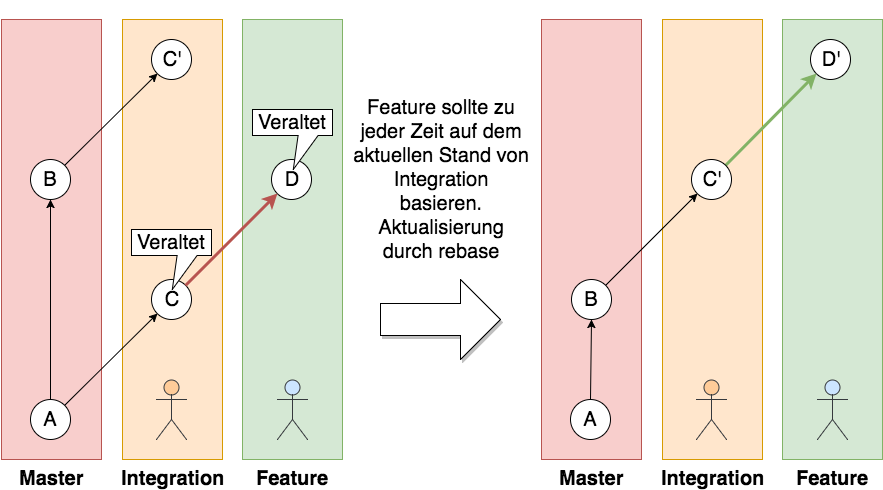
\includegraphics[width=\textwidth]{veraltete_branches}
    \end{center}
  \end{figure}
\end{frame}


\againframe<handout:0>{fragen}


\section{Arbeiten mit Git}


\subsection{Repositories organisieren}


\begin{frame}
  \frametitle{Repositories organisieren}
  \framesubtitle{Repositories beliebig verknüpfen}
  \begin{columns}[onlytextwidth]
    \begin{column}{0.5\textwidth}
      \begin{figure}
        \begin{center}
          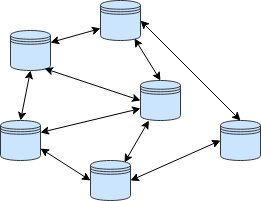
\includegraphics[width=\textwidth]{git_mesh}
        \end{center}
      \end{figure}
    \end{column}
    \begin{column}{0.5\textwidth}
    \begin{itemize}
      \item<+-> Repositories existieren prinzipell unabhängig
      \item<+-> Können mit Prozesseregel organisiert werden
      \item<+-> Daten könne mit Push, Pull oder Patch ausgetauscht werden
    \end{itemize}
    \end{column}
  \end{columns}
\end{frame}


\begin{frame}
  \frametitle{Repositories organisieren}
  \framesubtitle{Protokolle}
  Git bietet einige Protokolle zur Datenübertragung
  \begin{itemize}
    \item git
    \item file
    \item ssh
    \item http
    \item mailto
  \end{itemize}

\end{frame}


\begin{frame}
  \frametitle{Repositories organisieren}
  \framesubtitle{Zentrales Rpositry}
  \begin{columns}[onlytextwidth]
    \begin{column}{0.5\textwidth}
    \begin{itemize}
      \item<+-> Zentrales Repository als gemeinsamen Stand
      \item<+-> Entwickler pushen und pullen beliebig aus Central
      \item<+-> Keine Kontrollinstanz
      \item<+-> Einfach umzusetzen asd dfsdf
    \end{itemize}
    \end{column}
      \begin{column}{0.5\textwidth}
        \begin{figure}
          \begin{center}
            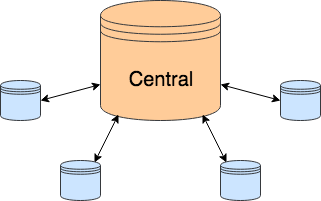
\includegraphics[width=\textwidth]{git_central}
          \end{center}
        \end{figure}
      \end{column}
  \end{columns}
\end{frame}


\begin{frame}
  \frametitle{Repositories organisieren}
  \framesubtitle{Zentrales Rpositry}
  \begin{columns}[onlytextwidth]
    \begin{column}{0.5\textwidth}
    \begin{itemize}
      \item<+-> Verteilte Verantwortung (Network of Trust)
      \item<+-> Verwalter betrachten verschiedene Scopes
      \item<+-> Hochflexibel
    \end{itemize}
    \end{column}
      \begin{column}{0.5\textwidth}
        \begin{figure}
          \begin{center}
            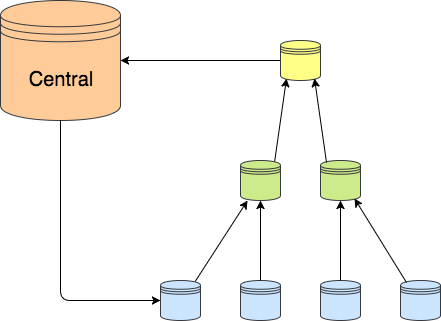
\includegraphics[width=\textwidth]{git_hierachy}
          \end{center}
        \end{figure}
      \end{column}
  \end{columns}
\end{frame}


\begin{frame}
  \frametitle{Repositories organisieren}
  \framesubtitle{Zentrales Rpositry}
  \begin{columns}[onlytextwidth]
    \begin{column}{0.49\textwidth}
    \begin{itemize}
      \item Continuous integration
      \item Automatische Tests
      \item Abnahme
      \item Einheitlicher Entwicklungsstand
      \item Releases
    \end{itemize}
    \end{column}
      \begin{column}{0.49\textwidth}
        \begin{figure}
          \begin{center}
            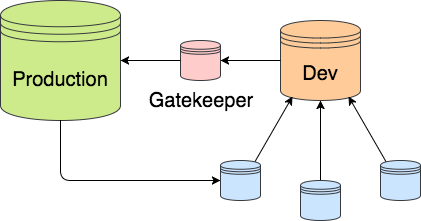
\includegraphics[width=\textwidth]{git_gatekeeper}
          \end{center}
        \end{figure}
      \end{column}
  \end{columns}
\end{frame}


\againframe<handout:0>{fragen}


\subsection{Git Cli}


\begin{frame}
  \frametitle{Git CLI}
  \framesubtitle{Warum CLI?}
  \begin{columns}[onlytextwidth]
    \begin{column}{0.49\textwidth}
    \begin{itemize}
      \item Use Git the Git way
      \item Umfangreicher Werkzeugkofer
      \item Schnell
      \item Zielsicher
      \item Stabil
    \end{itemize}
    \end{column}
      \begin{column}{0.49\textwidth}
        \begin{figure}
          \begin{center}
            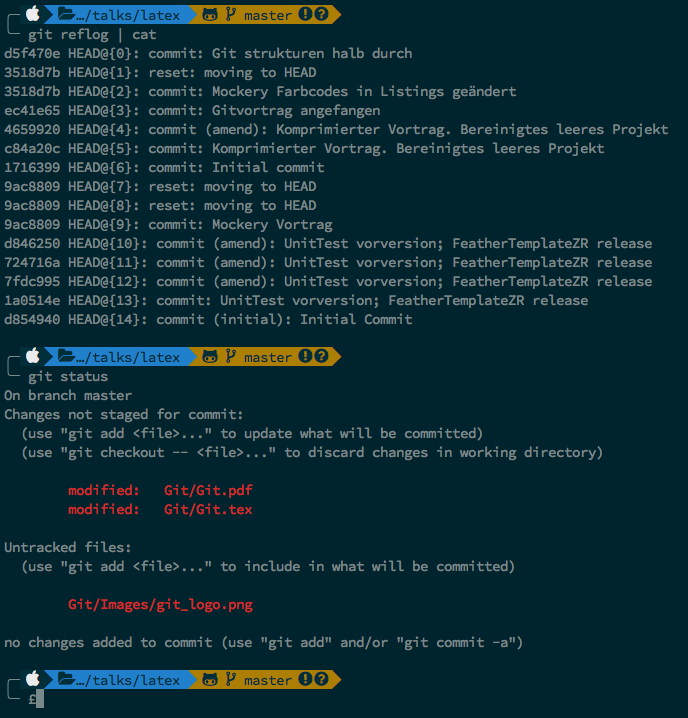
\includegraphics[width=\textwidth]{git_client}
          \end{center}
        \end{figure}
      \end{column}
  \end{columns}
\end{frame}


\begin{frame}
  \frametitle{Git CLI}
  \framesubtitle{Adressierung von Git-Objekten}
  \begin{columns}[onlytextwidth]

  \begin{column}{0.45\textwidth}
  \begin{block}{commit-ish}
    A commit object or an object that can be recursively dereferenced to a commit object.
    \begin{itemize}
      \item a commit object
      \item a tag object that points to a commit object
    \end{itemize}
  \end{block}
  \end{column}

    \begin{column}{0.45\textwidth}
    \begin{figure}
      \begin{center}
        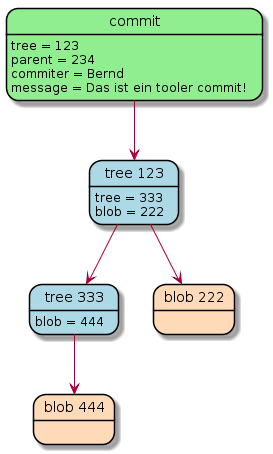
\includegraphics[height=6cm]{commit}
      \end{center}
    \end{figure}
    \end{column}

  \end{columns}
\end{frame}


\begin{frame}
  \frametitle{Git CLI}
  \framesubtitle{Adressierung von Git-Objekten}
  \begin{columns}[onlytextwidth]

  \begin{column}{0.45\textwidth}
  \begin{block}{tree-ish}
    A tree object or an object that can be recursively dereferenced to a tree object.
    \begin{itemize}
      \item a commit-ish \\(tree of top directory)
      \item a tree object
      \item a tag object that points to a tree object
    \end{itemize}
  \end{block}
  \end{column}

    \begin{column}{0.45\textwidth}
    \begin{figure}
      \begin{center}
        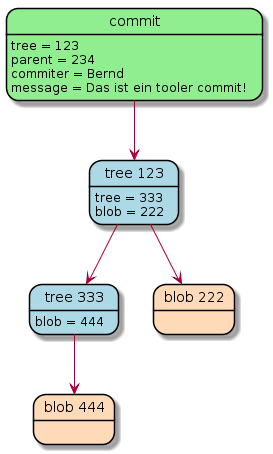
\includegraphics[height=6cm]{commit}
      \end{center}
    \end{figure}
    \end{column}

  \end{columns}
\end{frame}


\begin{frame}
  \frametitle{Git CLI}
  \framesubtitle{Adressierung von Git-Objekten}

  \begin{tabular}{ l | l }
  commit-ish & Example \\ \hline
  \lstinline|<sha1>                | & \lstinline|dae86e1950b1277e545cee180551750029cfe735|  \\
  \lstinline|<describeOutput>      | & \lstinline|v1.7.4.2-679-g3bee7fb| \\
  \lstinline|<refname>             | & \lstinline|master, heads/master, refs/heads/master| \\
  \lstinline|<refname>@\{<date>\}  | & \lstinline|master@\{yesterday\}, HEAD@\{5 minutes\}| \\
  \lstinline|<refname>@\{<n>\}     | & \lstinline|master@\{1\}| \\
  \lstinline|@\{<n>\}              | & \lstinline|@\{1\}| \\
  \lstinline|@\{-<n>\}             | & \lstinline|@\{-1\}| \\
  \lstinline|<refname>@\{upstream\}| & \lstinline|master@\{upstream\}, @\{u\}| \\
  \lstinline|<rev>^                | & \lstinline|HEAD^, v1.5.1^0| \\
  \lstinline|<rev>~<n>             | & \lstinline|master~3| \\
  \lstinline|<rev>^\{<type>\}      | & \lstinline|v0.99.8^\{commit\}| \\
  \lstinline|<rev>^\{\}            | & \lstinline|v0.99.8^\{\}| \\
  \lstinline|<rev>^\{/<text>\}     | & \lstinline|HEAD^\{/fix nasty bug\}| \\
  \lstinline|:/<text>              | & \lstinline|:/fix nasty bug|
  \end{tabular}

  \href{https://www.kernel.org/pub/software/scm/git/docs/gitrevisions.html\#_specifying_revisions}{\beamergotobutton{Git Dokumentation}}

\end{frame}


\againframe<handout:0>{fragen}


\begin{frame}
  \frametitle{Reflog}
  \framesubtitle{The easy way out}
  \begin{columns}[onlytextwidth,b]
    \begin{column}{0.48\textwidth}
      {\Large git reflog} \href{https://git-scm.com/docs/git-reflog}{\beamergotobutton{Git Dokumentation}}
      \vspace{1em}
      \begin{itemize}
        \item Historie der letzten Git-Operationen
        \item Commit-ish benutzen um zum Stand zurück zu kehren
      \end{itemize}
      \begin{exampleblock}{}
        \lstinline|git reset --hard HEAD@\{5\}|
      \end{exampleblock}
    \end{column}
    \begin{column}{0.48\textwidth}
      \begin{figure}
        \begin{center}
          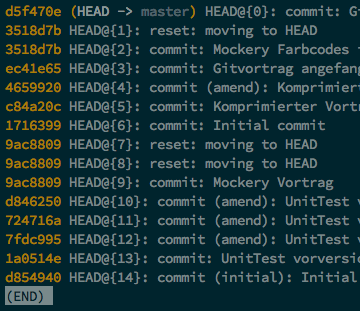
\includegraphics[width=\textwidth]{git_reflog}
        \end{center}
      \end{figure}
    \end{column}
  \end{columns}

\end{frame}


\begin{frame}
  \frametitle{Status}
  \framesubtitle{Status des aktuellen Workspace}
  \begin{columns}[onlytextwidth,b]
    \begin{column}{0.48\textwidth}
      {\Large git status} \href{https://git-scm.com/docs/git-status}{\beamergotobutton{Git Dokumentation}}
      \vspace{1em}
      \begin{itemize}
        \item Working mode \\
        (Rebasing, Merging \dots)
        \item Branch, Remotes
        \item Staged, Unstaged
      \end{itemize}
      \begin{exampleblock}{}
        \lstinline|git status| \\
        \vspace{1em}
        \lstinline|git status -sb \# aka STFU-Mode|
      \end{exampleblock}
    \end{column}
    \begin{column}{0.48\textwidth}
      \begin{figure}
        \begin{center}
          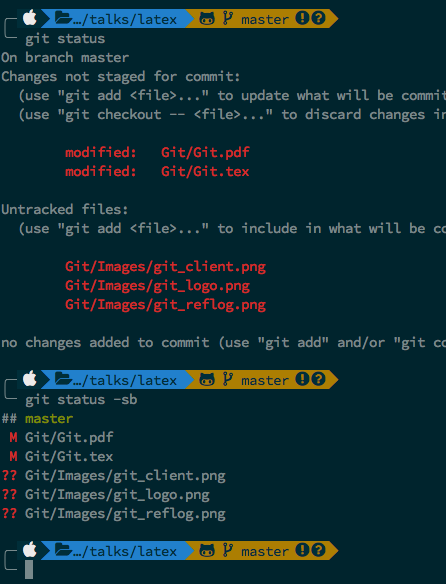
\includegraphics[width=\textwidth]{git_status}
        \end{center}
      \end{figure}
    \end{column}
  \end{columns}

\end{frame}


\begin{frame}
  \frametitle{Add}
  \framesubtitle{Dateien stagen}
  \begin{columns}[onlytextwidth,b]
    \begin{column}{0.48\textwidth}
      {\Large git add} \href{https://git-scm.com/docs/git-add}{\beamergotobutton{Git Dokumentation}}
      \vspace{1em}
      \begin{itemize}
        \item Fügt unbekannte Dateien zum index hinzu
        \item Staged Änderungen an bekannten Datien
      \end{itemize}
      \begin{exampleblock}{}
        \lstinline|git add NewFile.php| \\
        \lstinline|git add --all| \\
        \vspace{1em}
        \lstinline|git add -i \# Interactive|
      \end{exampleblock}
    \end{column}
    \begin{column}{0.48\textwidth}
      \begin{figure}
        \begin{center}
          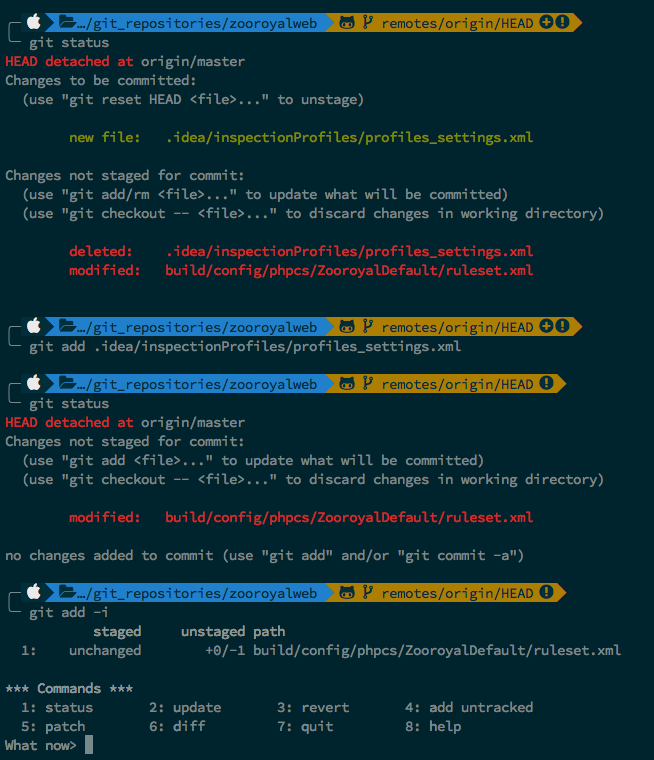
\includegraphics[width=\textwidth]{git_add}
        \end{center}
      \end{figure}
    \end{column}
  \end{columns}

\end{frame}


\begin{frame}
  \frametitle{Remove/Move}
  \framesubtitle{Dateien entfernen und verschieben}
  \begin{columns}[onlytextwidth,b]
    \begin{column}{0.48\textwidth}
      {\Large git rm / git mv} \href{https://git-scm.com/docs/git-rm}{\beamergotobutton{Git Dokumentation}}
      \vspace{1em}
      \begin{itemize}
        \item Git-Historie pflegen
      \end{itemize}
      \begin{exampleblock}{}
        \lstinline|git rm NewFile.php| \\
        \lstinline|git mv NFile.php NewFile.php| \\
      \end{exampleblock}
    \end{column}
    \begin{column}{0.48\textwidth}
      \begin{figure}
        \begin{center}
          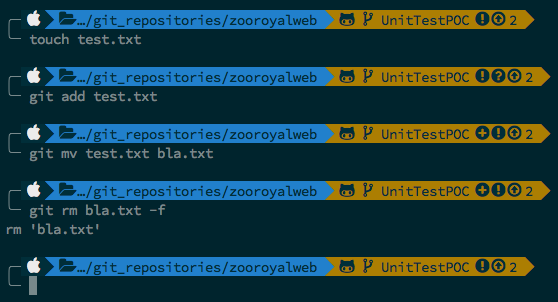
\includegraphics[width=\textwidth]{git_rm_mv}
        \end{center}
      \end{figure}
    \end{column}
  \end{columns}

\end{frame}


\begin{frame}[fragile]
  \frametitle{Checkout}
  \framesubtitle{Branches und Datein auschecken}
  \begin{columns}[onlytextwidth,b]
    \begin{column}{0.48\textwidth}
      {\Large git checkout} \href{https://git-scm.com/docs/git-checkout}{\beamergotobutton{Git Dokumentation}}\\
      \vspace{1em}
      Stellt Git-Objekte im Workspace bereit
      \begin{exampleblock}{}
        \begin{lstlisting}
# checkout branch
git checkout master
# create and checkout branch
git checkout -b new_Branch
# checkout remote branch at date
git checkout origin/master@{yesterday}
# checkout single file
git checkout <commit-ish> -- <file_path>
# checkout last used branch
git checkout - # alt: @{-1}
        \end{lstlisting}
      \end{exampleblock}
    \end{column}
    \begin{column}{0.48\textwidth}
      \begin{figure}
        \begin{center}
          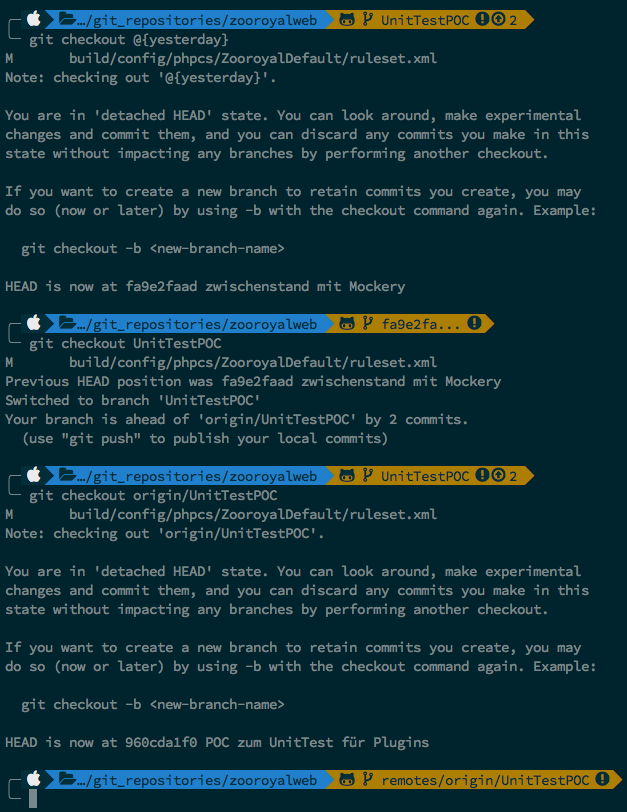
\includegraphics[width=\textwidth]{git_checkout}
        \end{center}
      \end{figure}
    \end{column}
  \end{columns}

\end{frame}


\begin{frame}[fragile]
  \frametitle{Log}
  \framesubtitle{Historie des aktuellen Workspaces}
  \begin{columns}[onlytextwidth,b]
    \begin{column}{0.48\textwidth}
      {\Large git log} \href{https://git-scm.com/docs/git-log}{\beamergotobutton{Git Dokumentation}} \\
      \vspace{1em}
      \begin{itemize}
        \item Zeigt die Historie
        \item Verschiedene Ansichten
        \item Durchsuchen
      \end{itemize}
      \begin{exampleblock}{}
        \begin{lstlisting}
git log
# detailed view
git log -p
# short view with graph
git log --graph --online
# grep message for pattern
git log --grep=Bugfix
# show commits since date
git log --since=yesterday
        \end{lstlisting}
      \end{exampleblock}
    \end{column}
    \begin{column}{0.48\textwidth}
      \begin{figure}
        \begin{center}
          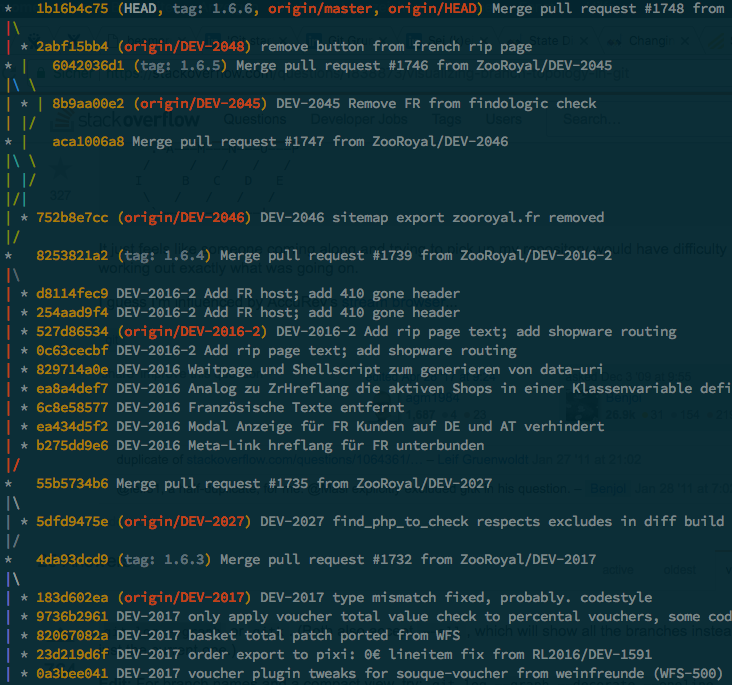
\includegraphics[width=\textwidth]{git_log}
        \end{center}
      \end{figure}
    \end{column}
  \end{columns}

\end{frame}


\begin{frame}[fragile]
  \frametitle{Diff}
  \framesubtitle{Unterschiede zwischen Commit-ishs}
  \begin{columns}[onlytextwidth,b]
    \begin{column}{0.48\textwidth}
      {\Large git diff} \href{https://git-scm.com/docs/git-diff}{\beamergotobutton{Git Dokumentation}} \\
      \vspace{1em}
      \begin{itemize}
        \item Zeigt unterschiede zwischen Commit-ishs
        \item Durchsuchen
      \end{itemize}
      \begin{exampleblock}{}
        \begin{lstlisting}
git diff
# only names of unmerged
git diff --name-only --diff-filter=U
# changed chars only
git diff --word-diff
# ignore whitespace
git diff HEAD~4..HEAD~2 -b
        \end{lstlisting}
      \end{exampleblock}
    \end{column}
    \begin{column}{0.48\textwidth}
      \begin{figure}
        \begin{center}
          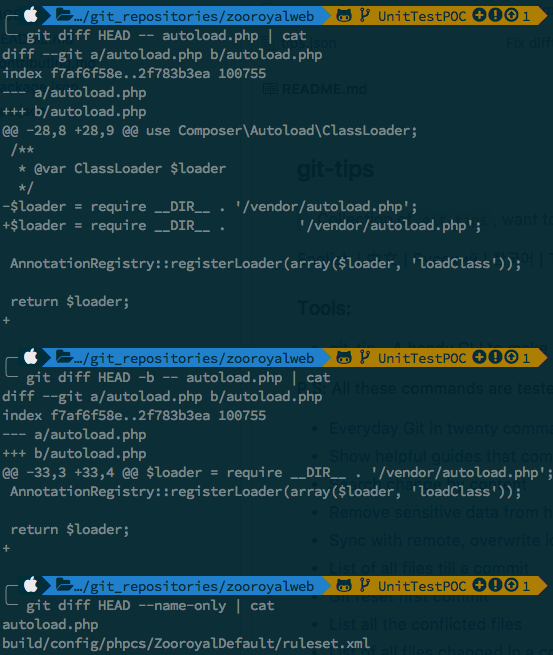
\includegraphics[width=\textwidth]{git_diff}
        \end{center}
      \end{figure}
    \end{column}
  \end{columns}

\end{frame}


\begin{frame}[fragile]
  \frametitle{Clean}
  \framesubtitle{Workspace aufräumen}
  \begin{columns}[onlytextwidth,b]
    \begin{column}{0.48\textwidth}
      {\Large git clean} \href{https://git-scm.com/docs/git-clean}{\beamergotobutton{Git Dokumentation}} \\
      \vspace{1em}
      \begin{itemize}
        \item Entfernt nicht indizierte Dateien
        \item .gitignore wird beachtet
      \end{itemize}
      \begin{exampleblock}{}
        \begin{lstlisting}
git clean
# deletes directories too
git clean -df
        \end{lstlisting}
      \end{exampleblock}
    \end{column}
    \begin{column}{0.48\textwidth}
      \begin{figure}
        \begin{center}
          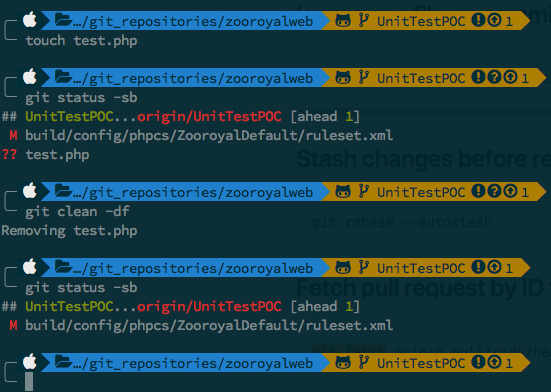
\includegraphics[width=\textwidth]{git_clean}
        \end{center}
      \end{figure}
    \end{column}
  \end{columns}

\end{frame}


\begin{frame}[fragile]
  \frametitle{Fetch}
  \framesubtitle{Informationen über Remotes einholen}
  \begin{columns}[onlytextwidth,b]
    \begin{column}{0.48\textwidth}
      {\Large git fetch} \href{https://git-scm.com/docs/git-fetch}{\beamergotobutton{Git Dokumentation}} \\
      \vspace{1em}
      Bezieht Refs von Remote-Reposioties

      \begin{exampleblock}{}
        \begin{lstlisting}
git fetch
# fetches a specific ref for branch
git fetch origin master:refs/remotes/origin/mymaster
        \end{lstlisting}
      \end{exampleblock}
    \end{column}
    \begin{column}{0.48\textwidth}
      \begin{figure}
        \begin{center}
          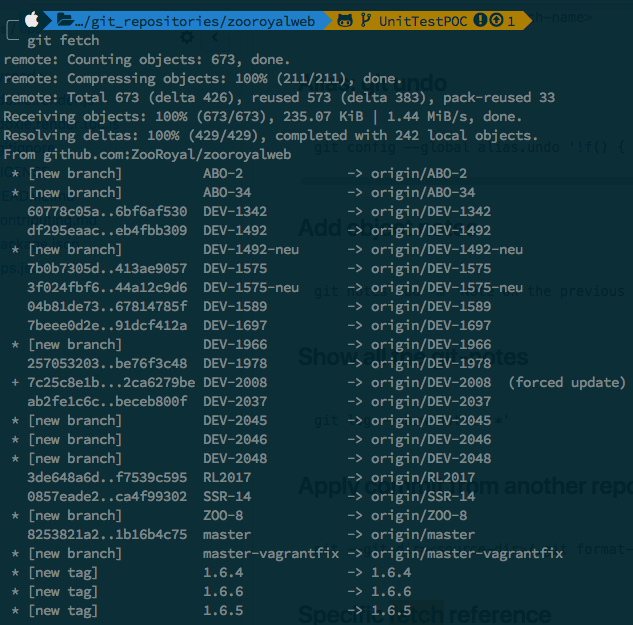
\includegraphics[width=\textwidth]{git_fetch}
        \end{center}
      \end{figure}
    \end{column}
  \end{columns}

\end{frame}


\begin{frame}[fragile]
  \frametitle{Merge}
  \framesubtitle{Zwei Branches zusammen führen}
  \begin{columns}[onlytextwidth,b]
    \begin{column}{0.48\textwidth}
      {\Large git merge} \href{https://git-scm.com/docs/git-merge}{\beamergotobutton{Git Dokumentation}} \\
      \begin{itemize}
        \item Führt zwei Branches zusammen
        \item Merge oder Fast-Forward
        \item Interaktiv
      \end{itemize}

      \begin{exampleblock}{}
        \begin{lstlisting}
# Pause before commit
git merge --no-commit Quellbranch
# Abort ongoing merge
git merge --abort
# Continue paused merge
git merge --continue
# Force non Fast-Forward
git merge -no-ff Quellbranch
        \end{lstlisting}
      \end{exampleblock}
    \end{column}
    \begin{column}{0.48\textwidth}
      \begin{figure}
        \begin{center}
          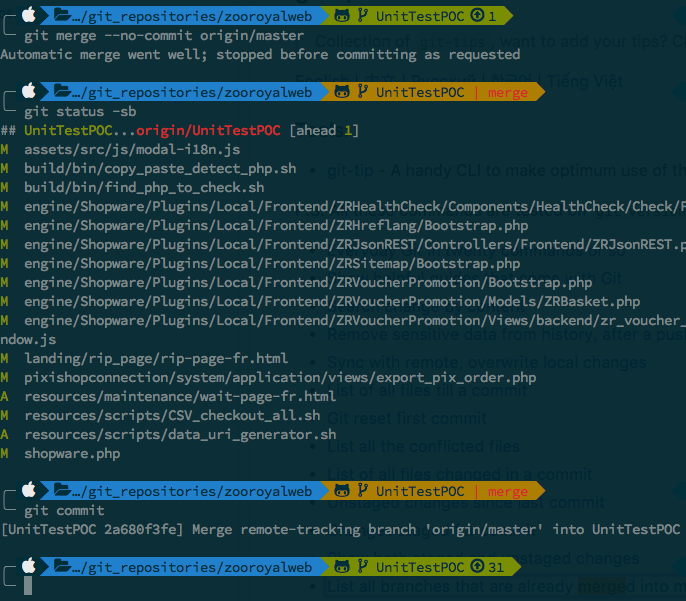
\includegraphics[width=\textwidth]{git_merge}
        \end{center}
      \end{figure}
    \end{column}
  \end{columns}

\end{frame}


\begin{frame}[fragile]
  \frametitle{Pull}
  \framesubtitle{Daten aus dem anderem Branch integrieren}
  \begin{columns}[onlytextwidth,b]
    \begin{column}{0.48\textwidth}
      {\Large git pull} \href{https://git-scm.com/docs/git-pull}{\beamergotobutton{Git Dokumentation}} \\
      \begin{itemize}
        \item Integriert Daten aus anderem Branch
        \item Fetch und merge
      \end{itemize}

      \begin{exampleblock}{}
        \begin{lstlisting}
# fetch + merge FETCH_HEAD
git pull
# pull ref from remote
git pull origin master
# fetch + rebase instead
git pull --rebase master
# Config always rebase
git config --global pull.rebase true

        \end{lstlisting}
      \end{exampleblock}
    \end{column}
    \begin{column}{0.48\textwidth}
      \begin{figure}
        \begin{center}
          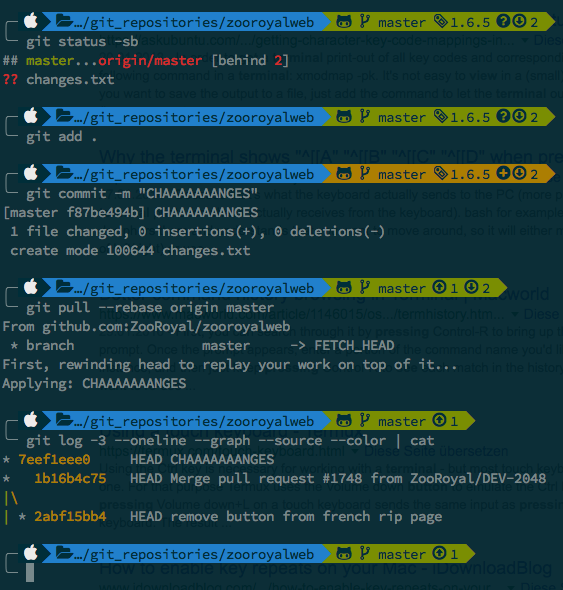
\includegraphics[width=\textwidth]{git_pull}
        \end{center}
      \end{figure}
    \end{column}
  \end{columns}

\end{frame}


\begin{frame}[fragile]
  \frametitle{Push}
  \framesubtitle{Daten in anderen Branch übertragen}
  \begin{columns}[onlytextwidth,b]
    \begin{column}{0.48\textwidth}
      {\Large git push} \href{https://git-scm.com/docs/git-push}{\beamergotobutton{Git Dokumentation}} \\
      \vspace{1em}
      Remote-Repository-Daten schreiben oder löschen
      \begin{exampleblock}{}
        \begin{lstlisting}
# force push to origin/branch
git push -f origin branch
# delete remote branch
git push origin :branch
# protected force push
git push --force-with-lease
        \end{lstlisting}
      \end{exampleblock}
    \end{column}
    \begin{column}{0.48\textwidth}
      \begin{figure}
        \begin{center}
          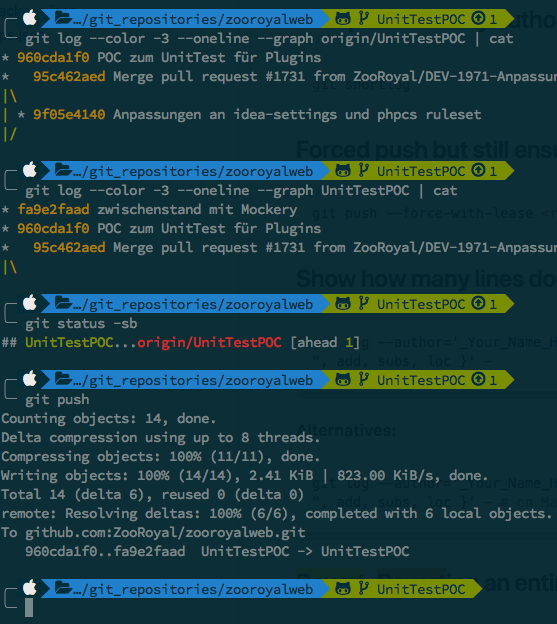
\includegraphics[width=\textwidth]{git_push}
        \end{center}
      \end{figure}
    \end{column}
  \end{columns}

\end{frame}


\begin{frame}[fragile]
  \frametitle{Revert}
  \framesubtitle{Änderungen mit sauberer History rückgängig}
  \begin{columns}[onlytextwidth,b]
    \begin{column}{0.48\textwidth}
      {\Large git revert} \href{https://git-scm.com/docs/git-revert}{\beamergotobutton{Git Dokumentation}} \\
      \vspace{1em}
      Erzeugt einen neuen Commit der Änderungen eines anderen Commits rückgängig macht
      \begin{exampleblock}{}
        \begin{lstlisting}
# undo <commit-ish>
git revert <commit-ish>
# undo merge
git revert -m 1 <commit-ish>
        \end{lstlisting}
      \end{exampleblock}
    \end{column}
    \begin{column}{0.48\textwidth}
      \begin{figure}
        \begin{center}
          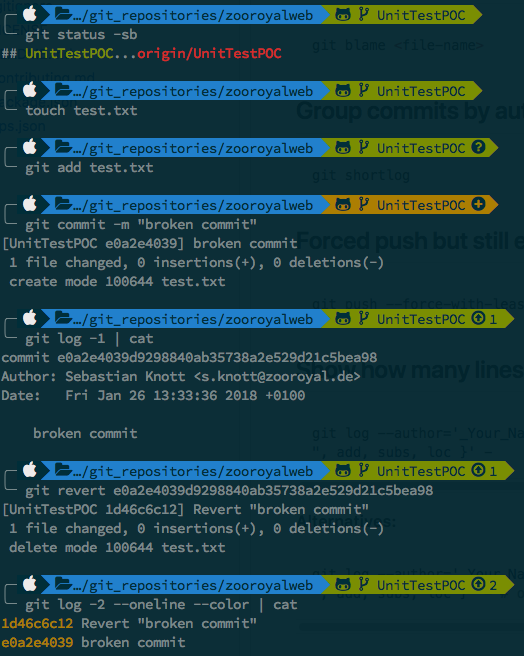
\includegraphics[width=\textwidth]{git_revert}
        \end{center}
      \end{figure}
    \end{column}
  \end{columns}

\end{frame}


\begin{frame}[fragile]
  \frametitle{Branch}
  \framesubtitle{Branches verwalten}
  \begin{columns}[onlytextwidth,b]
    \begin{column}{0.48\textwidth}
      {\Large git branch} \href{https://git-scm.com/docs/git-branch}{\beamergotobutton{Git Dokumentation}} \\
      \vspace{1em}
      \begin{itemize}
        \item Durchsuchen
        \item Hinzufügen
        \item Löschen
      \end{itemize}
      \begin{exampleblock}{}
        \begin{lstlisting}
# list merged branchesNN
git branch --merged master
# delete local MyBranch
git branch -d MyBranch
# list info of local branches
git branch -vv
        \end{lstlisting}
      \end{exampleblock}
    \end{column}
    \begin{column}{0.48\textwidth}
      \begin{figure}
        \begin{center}
          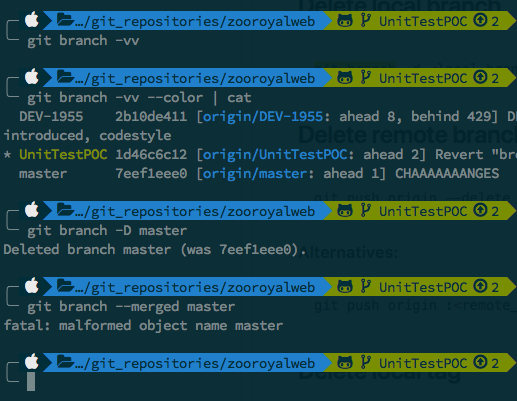
\includegraphics[width=\textwidth]{git_branch}
        \end{center}
      \end{figure}
    \end{column}
  \end{columns}

\end{frame}


\begin{frame}
  \frametitle{Weiteres}
  \begin{itemize}
    \item \href{https://try.github.io}{Einsteigerkurs von GitHub}
    \item \href{https://rogerdudler.github.io/git-guide/index.de.html}{Roger Dudlers Git Guide}
    \item \href{https://github.com/git-tips/tips}{Git Tricks}
  \end{itemize}


\end{frame}


\begin{frame}[plain]
 \begin{columns}[onlytextwidth]
   \begin{column}{0.5\textwidth}
     \begin{center}
        
\includegraphics[width=0.5\textwidth]{danke}
     \end{center}
   \end{column}
   \begin{column}{0.5\textwidth}
     Danke für eure Aufmerksamkeit!
   \end{column}
 \end{columns}
\end{frame}

%-------------------------------------------------------
% HELPER PAGES
%-------------------------------------------------------

\appendix

\begin{frame}<handout:0>[label=5minPause]
  \frametitle{Pause}
  \framesubtitle{5 Minuten Pause}
  \begin{figure}
    \begin{center}
      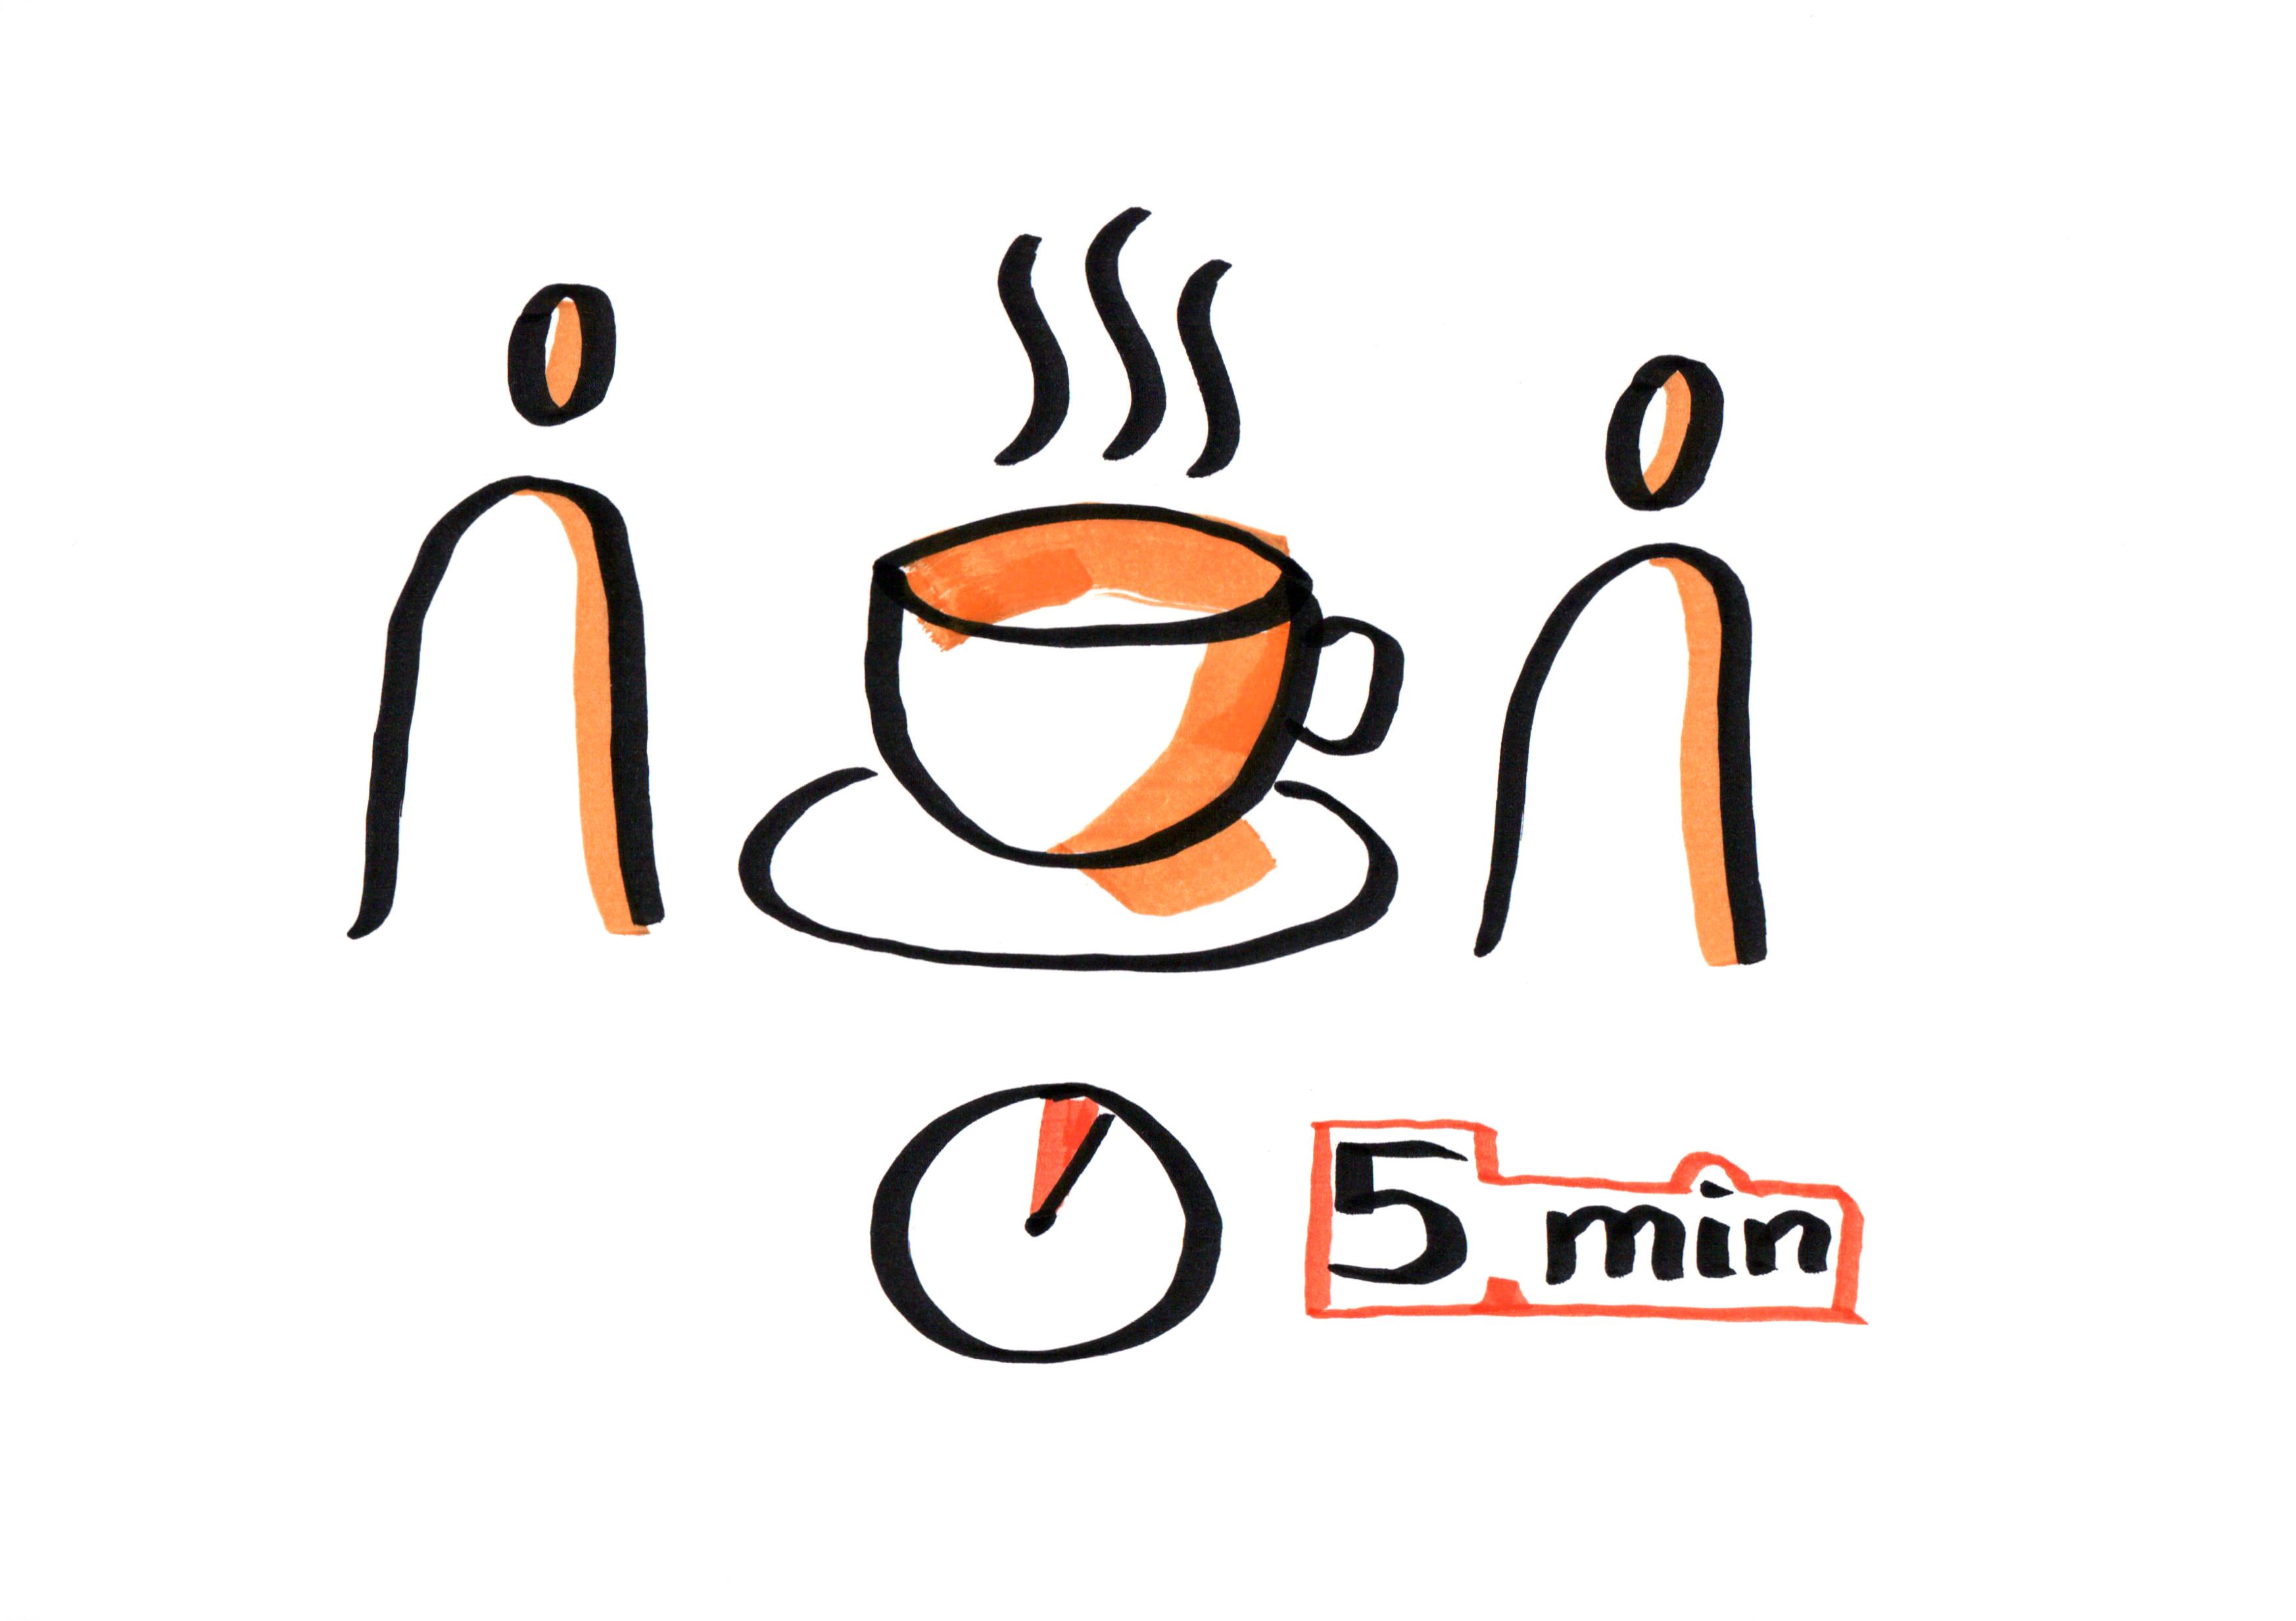
\includegraphics[height=4cm]{pause-5-min}
    \end{center}
  \end{figure}
\end{frame}



\begin{frame}<handout:0>[label=10minPause]
  \frametitle{Pause}
  \framesubtitle{10 Minuten Pause}
  \begin{figure}
    \begin{center}
      
\includegraphics[height=4cm]{pause-10-min}
    \end{center}
  \end{figure}
\end{frame}



\begin{frame}<handout:0>[label=pause]
  \frametitle{Pause}
  \framesubtitle{Pause}
  \begin{figure}
    \begin{center}
      
\includegraphics[height=4cm]{pause}
    \end{center}
  \end{figure}
\end{frame}



\begin{frame}<handout:0>[label=fragen]
  \frametitle{Fragen}
  \framesubtitle{Fragen?}
  \begin{figure}
    \begin{center}
      
\includegraphics[height=4cm]{fragen}
    \end{center}
  \end{figure}
\end{frame}



\end{document}
